\section{Системное проектирование}
\label{sec:arch}

После тщательного изучения предметной области, постановки целей и выделения задач дипломного проектирования, была
разработана структурная схема системы функционального контроля ТС КМУ артиллерийского дивизиона.
Система разделена на несколько слабо связанных модулей.
Данная система представляет собой клиент серверную архитектуру~\cite{cl_s},
где АРМ является сервером и осуществляет проверку клиентов -- подключенных устройств.

\begin{figure}[ht]
	\centering
	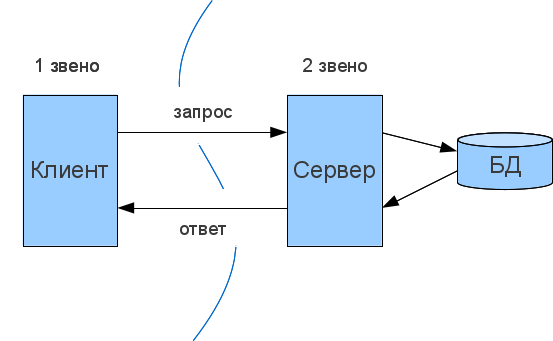
\includegraphics[scale=1.1]{client-s}
	\caption{Архитектура клиент-сервер~\cite{cl_s}}
	\label{fig:sec_arch:client}
\end{figure}

В системе имеются следующие блоки:
\begin{itemize}
	\item управляющий модуль;
	\item блок тестирования ЛВС;
	\item блок тестирования метеостанции;
	\item блок тестирования навигационной системы;
	\item блок тестирования радиостанции;
	\item блок журналирования;
	\item блок тестирования прибора наблюдения разведчика;
	\item блок тестирования лазерного целеуказателя-дальномера;
	\item блок тестирования принтера.
\end{itemize}

Данные модули являются достаточно независимыми друг от друга.\break Вследствие того, что система проводит тестирования
множества различных
устройств, модули, работающие с периферийными устройствами, имеют\break связь лишь с управляющим модулем.

Структурная схема, с изображением всех блоков и связей между ними, приведена на чертеже ГУИР.400201.065 С1.

Рассмотрим подробнее функциональные блоки системы.

\textit{Управляющий модуль} занимается коммуникацией с другими блоками. Модуль инициирует тестирование технических
средств, осуществляет прием и вывод информации от блоков, работающих с периферией. Также данный модуль отвечает за
взаимодействие с пользователем посредством элементов графического интерфейса. Функции визуализации процесса тестирования
также реализованы в модуле.

Данный модуль общается с другими блоками путем вызова публично доступных методов блоков.

Взаимодействие с пользователем осуществляется с помощью графического интерфейса, основанного на Qt виджетах. Передача
управления другим блокам осуществляется с помощью команд контекстного меню и кнопок графического интерфейса.

Управляющий блок позволяет:
\begin{itemize}
	\item инициировать тестирование ЛВС;
	\item инициировать тестирование метеостанции;
	\item инициировать тестирование принтера;
	\item инициировать тестирование радиостанции;
	\item инициировать тестирование системы навигации;
	\item инициировать тестирование прибора наблюдения разведчика;
	\item инициировать тестирование лазерного целеуказателя-дальномера;
	\item осуществлять логгирование результатов тестирования;
	\item осуществлять визуализацию процесса тестирования.
	\item осуществлять вывод результатов тестирования на экран либо на бумагу.
\end{itemize}

Посредством элементов графического интерфейса данный модуль может осуществлять передачу управления программе,
выполняющей отображение содержимого журнала тестирования.

\textit{Блок тестирования специального принтера} осуществляет проверку работоспособности принтера экипажа. Данный модуль
позволяет проверить корректность настроек подключения принтера, проверить уровень чернил и настройки параметров печати
путем печати тестовой
страницы.

\textit{Блок тестирования и настройки ЛВС} позволяет производить проверку состояния подключенных к ЛВС АРМ путем
отправки ping сообщений.

Все АРМ внутри КМУ подключены к ЛВС, также к сети подключены и такие устройства как радиостанции и навигационная система..
Машина управления также может связаться с другими машинами комплекса, используя ЛВС.

\textit{Блок тестирования навигационной системы} позволяет провести функциональный контроль подключенных к АРМ устройств
навигации.

Комплексная навигационная система состоит из следующих устройств:
\begin{itemize}
	\item бесплатформенная навигационная система(БИНС);
	\item блок измерительный спутниковый (БИС);
	\item датчик пути цифровой(ДПЦ).
\end{itemize}

Напрямую система общается лишь с БИНС. Обмен информацией с БИС и ДПЦ идет через БИНС.

Блок предоставляет следующую информацию и данные в процессе тестирования:
\begin{itemize}
		\item модуль скорости;
		\item пройденный путь;
		\item источник начальных координат;
		\item углы ориентации;
		\item текущие координаты;
		\item используемая системы отсчета высоты;
		\item текущее время;
		\item единицы измерения высоты;
		\item достоверность текущих координат.
\end{itemize}


\textit{Блок тестирования радиостанции} занимается тестированием средств радиосвязи.

В машинах КМУ установлено несколько различных типов радиостанций, общение с которыми имеет определенные отличия.
Радиостанции имеют
различный тип внутреннего устройства, различный форм фактор, различный диапазон для передачи данных.

Данный блок позволяет проводить тестирование всех подключенных радиостанций, независимо от их типа и форм фактора.

Блок предоставляет следующую информацию и данные в процессе тестирования:
\begin{itemize}
		\item корректность настроек подключения;
		\item параметры подключения прибора;
		\item тип радиостанции;
		\item текущие частоты приема и передачи;
		\item выходная мощность радиостанции;
		\item состояние шумоподавителя;
		\item номер канала;
		\item собственный адрес станции.
\end{itemize}

\textit{Блок тестирования метеостанции} позволяет проводить тестирование работы метеостанции, которая имеется во
всех КМУ.
Блок осуществляет проверку корректности параметров и настроек подключения прибора, получает различную
информацию о
состоянии прибора. Модуль также осуществляет обработку и анализ данных, полученных прибором в ходе работы.

Блок предоставляет следующую информацию и данные в процессе тестирования:
\begin{itemize}
		\item корректность настроек подключения;
		\item параметры подключении прибора;
		\item адрес устройства;
		\item скорость ветра;
		\item направление ветра;
		\item уровень атмосферного давления;
		\item текущая температура воздуха;
		\item уровень атмосферной влажности;
		\item информация о количестве и интенсивности осадков в виде дождя;
		\item информация о количестве и интенсивности осадков в виде града;
		\item данные о напряжении различных компонентов устройства.
\end{itemize}

\textit{Блок журналирования} осуществляет логгирование результатов тестирования, а также предоставляет интерфейс для
просмотра данной информации.

Модуль блока, отвечающий за сохранение результатов тестирования в журнал, осуществляет хранение данных в следующей
иерархии:
\begin{enum}
	\item Результаты тестирования работы произвольного устройства.
	\item Группа записей, полученная в течении дня.
	\item Группа записей, содержащая результаты тестирования устройств, собранные за месяц.
\end{enum}

Для хранения данной информации был выбран формат JSON. Выбор данного формата хранения данных обусловлен тем, что данные
имеют сложную иерархическую структуру. Также несомненными достоинствами данного формата является простой формат
хранения данных, файл с результатами тестирования может быть легко прочитан пользователем, потому что является простым
текстовым файлом. Данный формат открывает возможности для передачи данных между разными платформами, что может оказаться
полезным в будущем. Также существуют множество библиотек, облегчающих работу с JSON.

Модуль блока, выполняющий отображения результатов тестирования, имеет следующие функции:
\begin{itemize}
	\item вывод записей за выбранный промежуток времени;
	\item наличие фильтрации по типу устройства;
	\item возможность отображения дополнительной информации при выводе результатов;
	\item возможность вывода информации лишь о результатах тестирования неисправных устройств.
\end{itemize}

\textit{Блок тестирования прибора наблюдения разведчика} осуществляет тестирование прибора наблюдения разведчика
<<Капонир>>. Блок осуществляет проверку корректности настроек и параметров подключения прибора, получает различную
информацию о
состоянии прибора. Блок также осуществляет обработку и анализ данных, полученных прибором в ходе работы.

Блок позволяет извлечь следующую информацию:
\begin{itemize}
		\item состояние прибора;
		\item заводской номер прибора;
		\item используемая система координат;
		\item текущие координаты;
		\item количество спутников;
		\item достоверность координатных данных;
		\item используемая спутниковая система;
		\item наличие ошибок в работе прибора.
\end{itemize}

\textit{Блок тестирования лазерного целеуказателя-дальномера} осуществляет тестирование лазерного
целеуказателя-дальномера 1Д22.
Блок осуществляет проверку корректности настроек и параметров подключения прибора, получает различную
информацию о
состоянии прибора. Модуль также осуществляет обработку и анализ данных, полученных прибором в ходе работы.

Блок позволяет извлечь следующую информацию:
\begin{itemize}
		\item корректность настроек подключения;
		\item параметры подключения прибора;
		\item состояние линии связи;
		\item корректность полученных данных.
\end{itemize}
